\documentclass[1p]{elsarticle_modified}
%\bibliographystyle{elsarticle-num}

%\usepackage[colorlinks]{hyperref}
%\usepackage{abbrmath_seonhwa} %\Abb, \Ascr, \Acal ,\Abf, \Afrak
\usepackage{amsfonts}
\usepackage{amssymb}
\usepackage{amsmath}
\usepackage{amsthm}
\usepackage{scalefnt}
\usepackage{amsbsy}
\usepackage{kotex}
\usepackage{caption}
\usepackage{subfig}
\usepackage{color}
\usepackage{graphicx}
\usepackage{xcolor} %% white, black, red, green, blue, cyan, magenta, yellow
\usepackage{float}
\usepackage{setspace}
\usepackage{hyperref}

\usepackage{tikz}
\usetikzlibrary{arrows}

\usepackage{multirow}
\usepackage{array} % fixed length table
\usepackage{hhline}

%%%%%%%%%%%%%%%%%%%%%
\makeatletter
\renewcommand*\env@matrix[1][\arraystretch]{%
	\edef\arraystretch{#1}%
	\hskip -\arraycolsep
	\let\@ifnextchar\new@ifnextchar
	\array{*\c@MaxMatrixCols c}}
\makeatother %https://tex.stackexchange.com/questions/14071/how-can-i-increase-the-line-spacing-in-a-matrix
%%%%%%%%%%%%%%%

\usepackage[normalem]{ulem}

\newcommand{\msout}[1]{\ifmmode\text{\sout{\ensuremath{#1}}}\else\sout{#1}\fi}
%SOURCE: \msout is \stkout macro in https://tex.stackexchange.com/questions/20609/strikeout-in-math-mode

\newcommand{\cancel}[1]{
	\ifmmode
	{\color{red}\msout{#1}}
	\else
	{\color{red}\sout{#1}}
	\fi
}

\newcommand{\add}[1]{
	{\color{blue}\uwave{#1}}
}

\newcommand{\replace}[2]{
	\ifmmode
	{\color{red}\msout{#1}}{\color{blue}\uwave{#2}}
	\else
	{\color{red}\sout{#1}}{\color{blue}\uwave{#2}}
	\fi
}

\newcommand{\Sol}{\mathcal{S}} %segment
\newcommand{\D}{D} %diagram
\newcommand{\A}{\mathcal{A}} %arc


%%%%%%%%%%%%%%%%%%%%%%%%%%%%%5 test

\def\sl{\operatorname{\textup{SL}}(2,\Cbb)}
\def\psl{\operatorname{\textup{PSL}}(2,\Cbb)}
\def\quan{\mkern 1mu \triangleright \mkern 1mu}

\theoremstyle{definition}
\newtheorem{thm}{Theorem}[section]
\newtheorem{prop}[thm]{Proposition}
\newtheorem{lem}[thm]{Lemma}
\newtheorem{ques}[thm]{Question}
\newtheorem{cor}[thm]{Corollary}
\newtheorem{defn}[thm]{Definition}
\newtheorem{exam}[thm]{Example}
\newtheorem{rmk}[thm]{Remark}
\newtheorem{alg}[thm]{Algorithm}

\newcommand{\I}{\sqrt{-1}}
\begin{document}

%\begin{frontmatter}
%
%\title{Boundary parabolic representations of knots up to 8 crossings}
%
%%% Group authors per affiliation:
%\author{Yunhi Cho} 
%\address{Department of Mathematics, University of Seoul, Seoul, Korea}
%\ead{yhcho@uos.ac.kr}
%
%
%\author{Seonhwa Kim} %\fnref{s_kim}}
%\address{Center for Geometry and Physics, Institute for Basic Science, Pohang, 37673, Korea}
%\ead{ryeona17@ibs.re.kr}
%
%\author{Hyuk Kim}
%\address{Department of Mathematical Sciences, Seoul National University, Seoul 08826, Korea}
%\ead{hyukkim@snu.ac.kr}
%
%\author{Seokbeom Yoon}
%\address{Department of Mathematical Sciences, Seoul National University, Seoul, 08826,  Korea}
%\ead{sbyoon15@snu.ac.kr}
%
%\begin{abstract}
%We find all boundary parabolic representation of knots up to 8 crossings.
%
%\end{abstract}
%\begin{keyword}
%    \MSC[2010] 57M25 
%\end{keyword}
%
%\end{frontmatter}

%\linenumbers
%\tableofcontents
%
\newcommand\colored[1]{\textcolor{white}{\rule[-0.35ex]{0.8em}{1.4ex}}\kern-0.8em\color{red} #1}%
%\newcommand\colored[1]{\textcolor{white}{ #1}\kern-2.17ex	\textcolor{white}{ #1}\kern-1.81ex	\textcolor{white}{ #1}\kern-2.15ex\color{red}#1	}

{\Large $\underline{12n_{0323}~(K12n_{0323})}$}

\setlength{\tabcolsep}{10pt}
\renewcommand{\arraystretch}{1.6}
\vspace{1cm}\begin{tabular}{m{100pt}>{\centering\arraybackslash}m{274pt}}
\multirow{5}{120pt}{
	\centering
	\includegraphics[width=112pt]{../../../GIT/diagram.site/Diagrams/png/2412_12n_0323.png}\\
\ \ \ A knot diagram\footnotemark}&
\allowdisplaybreaks
\textbf{Linearized knot diagam} \\
\cline{2-2}
 &
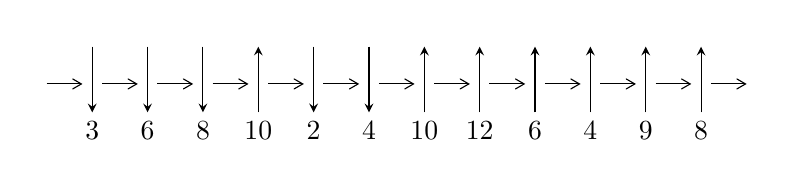
\begin{tikzpicture}[x=20pt, y=17pt]
	% nodes
	\node (C0) at (0, 0) {};
	\node (C1) at (1, 0) {};
	\node (C1U) at (1, +1) {};
	\node (C1D) at (1, -1) {3};

	\node (C2) at (2, 0) {};
	\node (C2U) at (2, +1) {};
	\node (C2D) at (2, -1) {6};

	\node (C3) at (3, 0) {};
	\node (C3U) at (3, +1) {};
	\node (C3D) at (3, -1) {8};

	\node (C4) at (4, 0) {};
	\node (C4U) at (4, +1) {};
	\node (C4D) at (4, -1) {10};

	\node (C5) at (5, 0) {};
	\node (C5U) at (5, +1) {};
	\node (C5D) at (5, -1) {2};

	\node (C6) at (6, 0) {};
	\node (C6U) at (6, +1) {};
	\node (C6D) at (6, -1) {4};

	\node (C7) at (7, 0) {};
	\node (C7U) at (7, +1) {};
	\node (C7D) at (7, -1) {10};

	\node (C8) at (8, 0) {};
	\node (C8U) at (8, +1) {};
	\node (C8D) at (8, -1) {12};

	\node (C9) at (9, 0) {};
	\node (C9U) at (9, +1) {};
	\node (C9D) at (9, -1) {6};

	\node (C10) at (10, 0) {};
	\node (C10U) at (10, +1) {};
	\node (C10D) at (10, -1) {4};

	\node (C11) at (11, 0) {};
	\node (C11U) at (11, +1) {};
	\node (C11D) at (11, -1) {9};

	\node (C12) at (12, 0) {};
	\node (C12U) at (12, +1) {};
	\node (C12D) at (12, -1) {8};
	\node (C13) at (13, 0) {};

	% arrows
	\draw[->,>={angle 60}]
	(C0) edge (C1) (C1) edge (C2) (C2) edge (C3) (C3) edge (C4) (C4) edge (C5) (C5) edge (C6) (C6) edge (C7) (C7) edge (C8) (C8) edge (C9) (C9) edge (C10) (C10) edge (C11) (C11) edge (C12) (C12) edge (C13) ;	\draw[->,>=stealth]
	(C1U) edge (C1D) (C2U) edge (C2D) (C3U) edge (C3D) (C4D) edge (C4U) (C5U) edge (C5D) (C6U) edge (C6D) (C7D) edge (C7U) (C8D) edge (C8U) (C9D) edge (C9U) (C10D) edge (C10U) (C11D) edge (C11U) (C12D) edge (C12U) ;
	\end{tikzpicture} \\
\hhline{~~} \\& 
\textbf{Solving Sequence} \\ \cline{2-2} 
 &
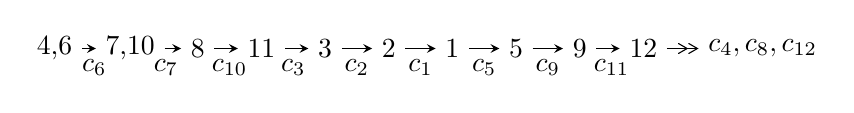
\begin{tikzpicture}[x=23pt, y=7pt]
	% node
	\node (A0) at (-1/8, 0) {4,6};
	\node (A1) at (17/16, 0) {7,10};
	\node (A2) at (17/8, 0) {8};
	\node (A3) at (25/8, 0) {11};
	\node (A4) at (33/8, 0) {3};
	\node (A5) at (41/8, 0) {2};
	\node (A6) at (49/8, 0) {1};
	\node (A7) at (57/8, 0) {5};
	\node (A8) at (65/8, 0) {9};
	\node (A9) at (73/8, 0) {12};
	\node (C1) at (1/2, -1) {$c_{6}$};
	\node (C2) at (13/8, -1) {$c_{7}$};
	\node (C3) at (21/8, -1) {$c_{10}$};
	\node (C4) at (29/8, -1) {$c_{3}$};
	\node (C5) at (37/8, -1) {$c_{2}$};
	\node (C6) at (45/8, -1) {$c_{1}$};
	\node (C7) at (53/8, -1) {$c_{5}$};
	\node (C8) at (61/8, -1) {$c_{9}$};
	\node (C9) at (69/8, -1) {$c_{11}$};
	\node (A10) at (11, 0) {$c_{4},c_{8},c_{12}$};

	% edge
	\draw[->,>=stealth]	
	(A0) edge (A1) (A1) edge (A2) (A2) edge (A3) (A3) edge (A4) (A4) edge (A5) (A5) edge (A6) (A6) edge (A7) (A7) edge (A8) (A8) edge (A9) ;
	\draw[->>,>={angle 60}]	
	(A9) edge (A10);
\end{tikzpicture} \\ 

\end{tabular} \\

\footnotetext{
The image of knot diagram is generated by the software ``\textbf{Draw programme}" developed by Andrew Bartholomew(\url{http://www.layer8.co.uk/maths/draw/index.htm\#Running-draw}), where we modified some parts for our purpose(\url{https://github.com/CATsTAILs/LinksPainter}).
}\phantom \\ \newline 
\centering \textbf{Ideals for irreducible components\footnotemark of $X_{\text{par}}$} 
 
\begin{align*}
I^u_{1}&=\langle 
-5.93292\times10^{96} u^{38}-8.20410\times10^{95} u^{37}+\cdots+4.97642\times10^{96} b-4.64235\times10^{97},\\
\phantom{I^u_{1}}&\phantom{= \langle  }-1.86317\times10^{97} u^{38}-7.56639\times10^{95} u^{37}+\cdots+4.97642\times10^{96} a-1.47890\times10^{98},\\
\phantom{I^u_{1}}&\phantom{= \langle  }u^{39}-27 u^{37}+\cdots+23 u-1\rangle \\
I^u_{2}&=\langle 
193 u^{12}+451 u^{11}+\cdots+b+265,\;-473 u^{12}-1171 u^{11}+\cdots+a-874,\\
\phantom{I^u_{2}}&\phantom{= \langle  }u^{13}+3 u^{12}- u^{11}-13 u^{10}-22 u^9-18 u^8+21 u^7+83 u^6+131 u^5+138 u^4+97 u^3+42 u^2+10 u+1\rangle \\
\\
\end{align*}
\raggedright * 2 irreducible components of $\dim_{\mathbb{C}}=0$, with total 52 representations.\\
\footnotetext{All coefficients of polynomials are rational numbers. But the coefficients are sometimes approximated in decimal forms when there is not enough margin.}
\newpage
\renewcommand{\arraystretch}{1}
\centering \section*{I. $I^u_{1}= \langle -5.93\times10^{96} u^{38}-8.20\times10^{95} u^{37}+\cdots+4.98\times10^{96} b-4.64\times10^{97},\;-1.86\times10^{97} u^{38}-7.57\times10^{95} u^{37}+\cdots+4.98\times10^{96} a-1.48\times10^{98},\;u^{39}-27 u^{37}+\cdots+23 u-1 \rangle$}
\flushleft \textbf{(i) Arc colorings}\\
\begin{tabular}{m{7pt} m{180pt} m{7pt} m{180pt} }
\flushright $a_{4}=$&$\begin{pmatrix}0\\u\end{pmatrix}$ \\
\flushright $a_{6}=$&$\begin{pmatrix}1\\0\end{pmatrix}$ \\
\flushright $a_{7}=$&$\begin{pmatrix}1\\u^2\end{pmatrix}$ \\
\flushright $a_{10}=$&$\begin{pmatrix}3.74399 u^{38}+0.152045 u^{37}+\cdots-535.809 u+29.7183\\1.19221 u^{38}+0.164860 u^{37}+\cdots-144.637 u+9.32870\end{pmatrix}$ \\
\flushright $a_{8}=$&$\begin{pmatrix}-12.4725 u^{38}-2.14316 u^{37}+\cdots+1137.22 u-63.9305\\0.330558 u^{38}+0.0519417 u^{37}+\cdots-31.6927 u+2.63188\end{pmatrix}$ \\
\flushright $a_{11}=$&$\begin{pmatrix}3.74399 u^{38}+0.152045 u^{37}+\cdots-535.809 u+29.7183\\1.24585 u^{38}+0.181271 u^{37}+\cdots-144.884 u+9.17665\end{pmatrix}$ \\
\flushright $a_{3}=$&$\begin{pmatrix}-8.97456 u^{38}-1.43150 u^{37}+\cdots+889.416 u-63.1649\\-1.50003 u^{38}-0.226969 u^{37}+\cdots+156.223 u-8.24024\end{pmatrix}$ \\
\flushright $a_{2}=$&$\begin{pmatrix}-10.4746 u^{38}-1.65847 u^{37}+\cdots+1045.64 u-71.4051\\-1.50003 u^{38}-0.226969 u^{37}+\cdots+156.223 u-8.24024\end{pmatrix}$ \\
\flushright $a_{1}=$&$\begin{pmatrix}-31.1624 u^{38}-4.81610 u^{37}+\cdots+3104.14 u-177.973\\-0.404984 u^{38}-0.0547518 u^{37}+\cdots+61.2052 u-2.70494\end{pmatrix}$ \\
\flushright $a_{5}=$&$\begin{pmatrix}-4.84811 u^{38}-0.726842 u^{37}+\cdots+500.726 u-13.4811\\2.04459 u^{38}+0.303981 u^{37}+\cdots-209.069 u+11.7457\end{pmatrix}$ \\
\flushright $a_{9}=$&$\begin{pmatrix}2.55178 u^{38}-0.0128147 u^{37}+\cdots-391.172 u+20.3896\\1.19221 u^{38}+0.164860 u^{37}+\cdots-144.637 u+9.32870\end{pmatrix}$ \\
\flushright $a_{12}=$&$\begin{pmatrix}11.7457 u^{38}+2.04459 u^{37}+\cdots-1039.19 u+61.0824\\0.0960919 u^{38}+0.00947475 u^{37}+\cdots-14.9880 u+0.00924794\end{pmatrix}$\\&\end{tabular}
\flushleft \textbf{(ii) Obstruction class $= -1$}\\~\\
\flushleft \textbf{(iii) Cusp Shapes $= 2.40504 u^{38}+0.306842 u^{37}+\cdots-347.511 u+22.5697$}\\~\\
\newpage\renewcommand{\arraystretch}{1}
\flushleft \textbf{(iv) u-Polynomials at the component}\newline \\
\begin{tabular}{m{50pt}|m{274pt}}
Crossings & \hspace{64pt}u-Polynomials at each crossing \\
\hline $$\begin{aligned}c_{1}\end{aligned}$$&$\begin{aligned}
&u^{39}+16 u^{38}+\cdots+329 u+1
\end{aligned}$\\
\hline $$\begin{aligned}c_{2},c_{5}\end{aligned}$$&$\begin{aligned}
&u^{39}+4 u^{38}+\cdots+15 u-1
\end{aligned}$\\
\hline $$\begin{aligned}c_{3}\end{aligned}$$&$\begin{aligned}
&u^{39}+10 u^{37}+\cdots+249 u-171
\end{aligned}$\\
\hline $$\begin{aligned}c_{4},c_{10}\end{aligned}$$&$\begin{aligned}
&u^{39}+u^{38}+\cdots+7 u-1
\end{aligned}$\\
\hline $$\begin{aligned}c_{6}\end{aligned}$$&$\begin{aligned}
&u^{39}-27 u^{37}+\cdots+23 u-1
\end{aligned}$\\
\hline $$\begin{aligned}c_{7}\end{aligned}$$&$\begin{aligned}
&u^{39}+2 u^{38}+\cdots-4549 u-567
\end{aligned}$\\
\hline $$\begin{aligned}c_{8},c_{11},c_{12}\end{aligned}$$&$\begin{aligned}
&u^{39}+4 u^{38}+\cdots-79 u-29
\end{aligned}$\\
\hline $$\begin{aligned}c_{9}\end{aligned}$$&$\begin{aligned}
&u^{39}+17 u^{37}+\cdots-4121 u-2447
\end{aligned}$\\
\hline
\end{tabular}\\~\\
\newpage\renewcommand{\arraystretch}{1}
\flushleft \textbf{(v) Riley Polynomials at the component}\newline \\
\begin{tabular}{m{50pt}|m{274pt}}
Crossings & \hspace{64pt}Riley Polynomials at each crossing \\
\hline $$\begin{aligned}c_{1}\end{aligned}$$&$\begin{aligned}
&y^{39}+24 y^{38}+\cdots+99345 y-1
\end{aligned}$\\
\hline $$\begin{aligned}c_{2},c_{5}\end{aligned}$$&$\begin{aligned}
&y^{39}-16 y^{38}+\cdots+329 y-1
\end{aligned}$\\
\hline $$\begin{aligned}c_{3}\end{aligned}$$&$\begin{aligned}
&y^{39}+20 y^{38}+\cdots-233145 y-29241
\end{aligned}$\\
\hline $$\begin{aligned}c_{4},c_{10}\end{aligned}$$&$\begin{aligned}
&y^{39}+49 y^{38}+\cdots-47 y-1
\end{aligned}$\\
\hline $$\begin{aligned}c_{6}\end{aligned}$$&$\begin{aligned}
&y^{39}-54 y^{38}+\cdots+67 y-1
\end{aligned}$\\
\hline $$\begin{aligned}c_{7}\end{aligned}$$&$\begin{aligned}
&y^{39}+40 y^{38}+\cdots+13389307 y-321489
\end{aligned}$\\
\hline $$\begin{aligned}c_{8},c_{11},c_{12}\end{aligned}$$&$\begin{aligned}
&y^{39}+22 y^{38}+\cdots-13189 y-841
\end{aligned}$\\
\hline $$\begin{aligned}c_{9}\end{aligned}$$&$\begin{aligned}
&y^{39}+34 y^{38}+\cdots-55732411 y-5987809
\end{aligned}$\\
\hline
\end{tabular}\\~\\
\newpage\flushleft \textbf{(vi) Complex Volumes and Cusp Shapes}
$$\begin{array}{c|c|c}  
\text{Solutions to }I^u_{1}& \I (\text{vol} + \sqrt{-1}CS) & \text{Cusp shape}\\
 \hline 
\begin{aligned}
u &= -0.994299 + 0.272414 I \\
a &= \phantom{-}0.463680 - 0.927259 I \\
b &= \phantom{-}1.018090 - 0.678656 I\end{aligned}
 & -0.629315 + 0.697668 I & -0.69777 + 1.96847 I \\ \hline\begin{aligned}
u &= -0.994299 - 0.272414 I \\
a &= \phantom{-}0.463680 + 0.927259 I \\
b &= \phantom{-}1.018090 + 0.678656 I\end{aligned}
 & -0.629315 - 0.697668 I & -0.69777 - 1.96847 I \\ \hline\begin{aligned}
u &= \phantom{-}0.649416 + 0.545046 I \\
a &= \phantom{-}0.543557 + 0.859256 I \\
b &= \phantom{-}0.932275 + 0.703931 I\end{aligned}
 & -0.04361 + 5.03289 I & -0.70677 - 5.74773 I \\ \hline\begin{aligned}
u &= \phantom{-}0.649416 - 0.545046 I \\
a &= \phantom{-}0.543557 - 0.859256 I \\
b &= \phantom{-}0.932275 - 0.703931 I\end{aligned}
 & -0.04361 - 5.03289 I & -0.70677 + 5.74773 I \\ \hline\begin{aligned}
u &= -1.003940 + 0.692341 I \\
a &= \phantom{-}0.328055 - 0.842205 I \\
b &= -1.78302 - 0.03484 I\end{aligned}
 & -1.32978 - 3.67485 I & \phantom{-0.000000 } 0 \\ \hline\begin{aligned}
u &= -1.003940 - 0.692341 I \\
a &= \phantom{-}0.328055 + 0.842205 I \\
b &= -1.78302 + 0.03484 I\end{aligned}
 & -1.32978 + 3.67485 I & \phantom{-0.000000 } 0 \\ \hline\begin{aligned}
u &= -0.639274 + 0.192301 I \\
a &= \phantom{-}0.756843 - 0.681921 I \\
b &= \phantom{-}0.300034 - 0.398633 I\end{aligned}
 & -1.39152 + 0.61829 I & -4.65215 - 1.06818 I \\ \hline\begin{aligned}
u &= -0.639274 - 0.192301 I \\
a &= \phantom{-}0.756843 + 0.681921 I \\
b &= \phantom{-}0.300034 + 0.398633 I\end{aligned}
 & -1.39152 - 0.61829 I & -4.65215 + 1.06818 I \\ \hline\begin{aligned}
u &= \phantom{-}0.593939 + 0.218894 I \\
a &= \phantom{-}0.976981 + 0.875107 I \\
b &= -1.005710 + 0.276370 I\end{aligned}
 & \phantom{-}1.53232 - 0.33929 I & \phantom{-}2.22376 + 1.90694 I \\ \hline\begin{aligned}
u &= \phantom{-}0.593939 - 0.218894 I \\
a &= \phantom{-}0.976981 - 0.875107 I \\
b &= -1.005710 - 0.276370 I\end{aligned}
 & \phantom{-}1.53232 + 0.33929 I & \phantom{-}2.22376 - 1.90694 I\\
 \hline 
 \end{array}$$\newpage$$\begin{array}{c|c|c}  
\text{Solutions to }I^u_{1}& \I (\text{vol} + \sqrt{-1}CS) & \text{Cusp shape}\\
 \hline 
\begin{aligned}
u &= \phantom{-}0.09219 + 1.41774 I \\
a &= \phantom{-}0.1177060 + 0.0003338 I \\
b &= -0.544510 - 0.762381 I\end{aligned}
 & \phantom{-}3.32998 + 1.36180 I & \phantom{-0.000000 } 0 \\ \hline\begin{aligned}
u &= \phantom{-}0.09219 - 1.41774 I \\
a &= \phantom{-}0.1177060 - 0.0003338 I \\
b &= -0.544510 + 0.762381 I\end{aligned}
 & \phantom{-}3.32998 - 1.36180 I & \phantom{-0.000000 } 0 \\ \hline\begin{aligned}
u &= -1.58355 + 0.07109 I \\
a &= \phantom{-}0.242255 + 1.000940 I \\
b &= \phantom{-}0.550049 + 1.295150 I\end{aligned}
 & -2.17716 + 0.58502 I & \phantom{-0.000000 } 0 \\ \hline\begin{aligned}
u &= -1.58355 - 0.07109 I \\
a &= \phantom{-}0.242255 - 1.000940 I \\
b &= \phantom{-}0.550049 - 1.295150 I\end{aligned}
 & -2.17716 - 0.58502 I & \phantom{-0.000000 } 0 \\ \hline\begin{aligned}
u &= \phantom{-}1.52238 + 0.49770 I \\
a &= -0.599371 - 0.810262 I \\
b &= \phantom{-}0.202320 - 1.285620 I\end{aligned}
 & -8.76356 + 1.01188 I & \phantom{-0.000000 } 0 \\ \hline\begin{aligned}
u &= \phantom{-}1.52238 - 0.49770 I \\
a &= -0.599371 + 0.810262 I \\
b &= \phantom{-}0.202320 + 1.285620 I\end{aligned}
 & -8.76356 - 1.01188 I & \phantom{-0.000000 } 0 \\ \hline\begin{aligned}
u &= -0.45538 + 1.56426 I \\
a &= -0.0753063 - 0.0530697 I \\
b &= -0.505804 + 0.964655 I\end{aligned}
 & \phantom{-}2.41500 + 4.97539 I & \phantom{-0.000000 } 0 \\ \hline\begin{aligned}
u &= -0.45538 - 1.56426 I \\
a &= -0.0753063 + 0.0530697 I \\
b &= -0.505804 - 0.964655 I\end{aligned}
 & \phantom{-}2.41500 - 4.97539 I & \phantom{-0.000000 } 0 \\ \hline\begin{aligned}
u &= -0.164690 + 0.303209 I \\
a &= \phantom{-}0.604983 + 0.898851 I \\
b &= \phantom{-}0.880121 + 0.762617 I\end{aligned}
 & -4.06684 + 2.90659 I & \phantom{-}6.73557 + 0.48460 I \\ \hline\begin{aligned}
u &= -0.164690 - 0.303209 I \\
a &= \phantom{-}0.604983 - 0.898851 I \\
b &= \phantom{-}0.880121 - 0.762617 I\end{aligned}
 & -4.06684 - 2.90659 I & \phantom{-}6.73557 - 0.48460 I\\
 \hline 
 \end{array}$$\newpage$$\begin{array}{c|c|c}  
\text{Solutions to }I^u_{1}& \I (\text{vol} + \sqrt{-1}CS) & \text{Cusp shape}\\
 \hline 
\begin{aligned}
u &= \phantom{-}1.65134 + 0.17017 I \\
a &= \phantom{-}0.210060 - 1.091670 I \\
b &= \phantom{-}0.59401 - 1.30121 I\end{aligned}
 & -2.82025 - 6.80896 I & \phantom{-0.000000 } 0 \\ \hline\begin{aligned}
u &= \phantom{-}1.65134 - 0.17017 I \\
a &= \phantom{-}0.210060 + 1.091670 I \\
b &= \phantom{-}0.59401 + 1.30121 I\end{aligned}
 & -2.82025 + 6.80896 I & \phantom{-0.000000 } 0 \\ \hline\begin{aligned}
u &= \phantom{-}0.316011\phantom{ +0.000000I} \\
a &= \phantom{-}1.69045\phantom{ +0.000000I} \\
b &= -0.597495\phantom{ +0.000000I}\end{aligned}
 & \phantom{-}1.11789\phantom{ +0.000000I} & \phantom{-}11.2670\phantom{ +0.000000I} \\ \hline\begin{aligned}
u &= \phantom{-}1.78797 + 0.23546 I \\
a &= -0.175928 - 1.026470 I \\
b &= \phantom{-}0.426419 - 1.281700 I\end{aligned}
 & -9.84094 - 3.14577 I & \phantom{-0.000000 } 0 \\ \hline\begin{aligned}
u &= \phantom{-}1.78797 - 0.23546 I \\
a &= -0.175928 + 1.026470 I \\
b &= \phantom{-}0.426419 + 1.281700 I\end{aligned}
 & -9.84094 + 3.14577 I & \phantom{-0.000000 } 0 \\ \hline\begin{aligned}
u &= \phantom{-}0.147459 + 0.018240 I \\
a &= \phantom{-}8.93744 + 0.12975 I \\
b &= -0.052132 - 0.818099 I\end{aligned}
 & \phantom{-}2.82165 + 0.44220 I & \phantom{-}0.165551 - 1.251212 I \\ \hline\begin{aligned}
u &= \phantom{-}0.147459 - 0.018240 I \\
a &= \phantom{-}8.93744 - 0.12975 I \\
b &= -0.052132 + 0.818099 I\end{aligned}
 & \phantom{-}2.82165 - 0.44220 I & \phantom{-}0.165551 + 1.251212 I \\ \hline\begin{aligned}
u &= \phantom{-}0.0757690 + 0.1010380 I \\
a &= -9.82475 + 6.73299 I \\
b &= \phantom{-}0.096930 - 1.077780 I\end{aligned}
 & \phantom{-}1.58306 + 6.33307 I & -2.17277 - 5.35202 I \\ \hline\begin{aligned}
u &= \phantom{-}0.0757690 - 0.1010380 I \\
a &= -9.82475 - 6.73299 I \\
b &= \phantom{-}0.096930 + 1.077780 I\end{aligned}
 & \phantom{-}1.58306 - 6.33307 I & -2.17277 + 5.35202 I \\ \hline\begin{aligned}
u &= -1.81753 + 0.76879 I \\
a &= -0.361839 + 0.599956 I \\
b &= \phantom{-}0.192205 + 1.129990 I\end{aligned}
 & -8.14778 + 2.96891 I & \phantom{-0.000000 } 0\\
 \hline 
 \end{array}$$\newpage$$\begin{array}{c|c|c}  
\text{Solutions to }I^u_{1}& \I (\text{vol} + \sqrt{-1}CS) & \text{Cusp shape}\\
 \hline 
\begin{aligned}
u &= -1.81753 - 0.76879 I \\
a &= -0.361839 - 0.599956 I \\
b &= \phantom{-}0.192205 - 1.129990 I\end{aligned}
 & -8.14778 - 2.96891 I & \phantom{-0.000000 } 0 \\ \hline\begin{aligned}
u &= \phantom{-}1.99569 + 0.16593 I \\
a &= \phantom{-}0.098834 + 0.938233 I \\
b &= \phantom{-}0.13027 + 2.53503 I\end{aligned}
 & -12.47920 - 1.55057 I & \phantom{-0.000000 } 0 \\ \hline\begin{aligned}
u &= \phantom{-}1.99569 - 0.16593 I \\
a &= \phantom{-}0.098834 - 0.938233 I \\
b &= \phantom{-}0.13027 - 2.53503 I\end{aligned}
 & -12.47920 + 1.55057 I & \phantom{-0.000000 } 0 \\ \hline\begin{aligned}
u &= -1.97927 + 0.41282 I \\
a &= \phantom{-}0.025347 - 0.879507 I \\
b &= -0.64583 - 1.82989 I\end{aligned}
 & -4.36641 + 6.38323 I & \phantom{-0.000000 } 0 \\ \hline\begin{aligned}
u &= -1.97927 - 0.41282 I \\
a &= \phantom{-}0.025347 + 0.879507 I \\
b &= -0.64583 + 1.82989 I\end{aligned}
 & -4.36641 - 6.38323 I & \phantom{-0.000000 } 0 \\ \hline\begin{aligned}
u &= \phantom{-}2.03401 + 0.41923 I \\
a &= -0.017030 + 0.900973 I \\
b &= -0.90609 + 1.73968 I\end{aligned}
 & -6.3597 - 13.3871 I & \phantom{-0.000000 } 0 \\ \hline\begin{aligned}
u &= \phantom{-}2.03401 - 0.41923 I \\
a &= -0.017030 - 0.900973 I \\
b &= -0.90609 - 1.73968 I\end{aligned}
 & -6.3597 + 13.3871 I & \phantom{-0.000000 } 0 \\ \hline\begin{aligned}
u &= -2.07024 + 0.28134 I \\
a &= -0.096745 + 0.760848 I \\
b &= \phantom{-}0.419131 + 1.090140 I\end{aligned}
 & -9.04262 + 0.68757 I & \phantom{-0.000000 } 0 \\ \hline\begin{aligned}
u &= -2.07024 - 0.28134 I \\
a &= -0.096745 - 0.760848 I \\
b &= \phantom{-}0.419131 - 1.090140 I\end{aligned}
 & -9.04262 - 0.68757 I & \phantom{-0.000000 } 0\\
 \hline 
 \end{array}$$\newpage\newpage\renewcommand{\arraystretch}{1}
\centering \section*{II. $I^u_{2}= \langle 193 u^{12}+451 u^{11}+\cdots+b+265,\;-473 u^{12}-1171 u^{11}+\cdots+a-874,\;u^{13}+3 u^{12}+\cdots+10 u+1 \rangle$}
\flushleft \textbf{(i) Arc colorings}\\
\begin{tabular}{m{7pt} m{180pt} m{7pt} m{180pt} }
\flushright $a_{4}=$&$\begin{pmatrix}0\\u\end{pmatrix}$ \\
\flushright $a_{6}=$&$\begin{pmatrix}1\\0\end{pmatrix}$ \\
\flushright $a_{7}=$&$\begin{pmatrix}1\\u^2\end{pmatrix}$ \\
\flushright $a_{10}=$&$\begin{pmatrix}473 u^{12}+1171 u^{11}+\cdots+7192 u+874\\-193 u^{12}-451 u^{11}+\cdots-2345 u-265\end{pmatrix}$ \\
\flushright $a_{8}=$&$\begin{pmatrix}-8 u^{12}-24 u^{11}+\cdots-273 u-46\\512 u^{12}+1280 u^{11}+\cdots+8192 u+1023\end{pmatrix}$ \\
\flushright $a_{11}=$&$\begin{pmatrix}473 u^{12}+1171 u^{11}+\cdots+7192 u+874\\-320 u^{12}-768 u^{11}+\cdots-4352 u-513\end{pmatrix}$ \\
\flushright $a_{3}=$&$\begin{pmatrix}-47 u^{12}-124 u^{11}+\cdots-1013 u-142\\- u^{12}-3 u^{11}+\cdots-42 u-9\end{pmatrix}$ \\
\flushright $a_{2}=$&$\begin{pmatrix}-48 u^{12}-127 u^{11}+\cdots-1055 u-151\\- u^{12}-3 u^{11}+\cdots-42 u-9\end{pmatrix}$ \\
\flushright $a_{1}=$&$\begin{pmatrix}122 u^{12}+318 u^{11}+\cdots+2113 u+256\\30 u^{12}+83 u^{11}+\cdots+719 u+103\end{pmatrix}$ \\
\flushright $a_{5}=$&$\begin{pmatrix}-103 u^{12}-278 u^{11}+\cdots-2217 u-303\\-8 u^{12}-23 u^{11}+\cdots-239 u-39\end{pmatrix}$ \\
\flushright $a_{9}=$&$\begin{pmatrix}666 u^{12}+1622 u^{11}+\cdots+9537 u+1139\\-193 u^{12}-451 u^{11}+\cdots-2345 u-265\end{pmatrix}$ \\
\flushright $a_{12}=$&$\begin{pmatrix}-39 u^{12}-109 u^{11}+\cdots-1000 u-151\\192 u^{12}+512 u^{11}+\cdots+3840 u+511\end{pmatrix}$\\&\end{tabular}
\flushleft \textbf{(ii) Obstruction class $= 1$}\\~\\
\flushleft \textbf{(iii) Cusp Shapes $= 1726 u^{12}+4212 u^{11}-4090 u^{10}-20161 u^9-26665 u^8-16081 u^7+45309 u^6+117921 u^5+159920 u^4+148350 u^3+83989 u^2+25167 u+3051$}\\~\\
\newpage\renewcommand{\arraystretch}{1}
\flushleft \textbf{(iv) u-Polynomials at the component}\newline \\
\begin{tabular}{m{50pt}|m{274pt}}
Crossings & \hspace{64pt}u-Polynomials at each crossing \\
\hline $$\begin{aligned}c_{1}\end{aligned}$$&$\begin{aligned}
&u^{13}-9 u^{12}+\cdots+14 u-1
\end{aligned}$\\
\hline $$\begin{aligned}c_{2}\end{aligned}$$&$\begin{aligned}
&u^{13}+3 u^{12}+\cdots-2 u-1
\end{aligned}$\\
\hline $$\begin{aligned}c_{3}\end{aligned}$$&$\begin{aligned}
&u^{13}- u^{12}+\cdots+4 u-1
\end{aligned}$\\
\hline $$\begin{aligned}c_{4}\end{aligned}$$&$\begin{aligned}
&u^{13}+6 u^{11}+\cdots+2 u-1
\end{aligned}$\\
\hline $$\begin{aligned}c_{5}\end{aligned}$$&$\begin{aligned}
&u^{13}-3 u^{12}+\cdots-2 u+1
\end{aligned}$\\
\hline $$\begin{aligned}c_{6}\end{aligned}$$&$\begin{aligned}
&u^{13}+3 u^{12}+\cdots+10 u+1
\end{aligned}$\\
\hline $$\begin{aligned}c_{7}\end{aligned}$$&$\begin{aligned}
&u^{13}+u^{12}+\cdots+2 u^2+1
\end{aligned}$\\
\hline $$\begin{aligned}c_{8}\end{aligned}$$&$\begin{aligned}
&u^{13}+3 u^{12}+\cdots+2 u+1
\end{aligned}$\\
\hline $$\begin{aligned}c_{9}\end{aligned}$$&$\begin{aligned}
&u^{13}- u^{12}+\cdots+4 u-1
\end{aligned}$\\
\hline $$\begin{aligned}c_{10}\end{aligned}$$&$\begin{aligned}
&u^{13}+6 u^{11}+\cdots+2 u+1
\end{aligned}$\\
\hline $$\begin{aligned}c_{11},c_{12}\end{aligned}$$&$\begin{aligned}
&u^{13}-3 u^{12}+\cdots+2 u-1
\end{aligned}$\\
\hline
\end{tabular}\\~\\
\newpage\renewcommand{\arraystretch}{1}
\flushleft \textbf{(v) Riley Polynomials at the component}\newline \\
\begin{tabular}{m{50pt}|m{274pt}}
Crossings & \hspace{64pt}Riley Polynomials at each crossing \\
\hline $$\begin{aligned}c_{1}\end{aligned}$$&$\begin{aligned}
&y^{13}- y^{12}+\cdots+30 y-1
\end{aligned}$\\
\hline $$\begin{aligned}c_{2},c_{5}\end{aligned}$$&$\begin{aligned}
&y^{13}-9 y^{12}+\cdots+14 y-1
\end{aligned}$\\
\hline $$\begin{aligned}c_{3}\end{aligned}$$&$\begin{aligned}
&y^{13}+3 y^{12}+\cdots-12 y-1
\end{aligned}$\\
\hline $$\begin{aligned}c_{4},c_{10}\end{aligned}$$&$\begin{aligned}
&y^{13}+12 y^{12}+\cdots-10 y-1
\end{aligned}$\\
\hline $$\begin{aligned}c_{6}\end{aligned}$$&$\begin{aligned}
&y^{13}-11 y^{12}+\cdots+16 y-1
\end{aligned}$\\
\hline $$\begin{aligned}c_{7}\end{aligned}$$&$\begin{aligned}
&y^{13}+11 y^{12}+\cdots-4 y-1
\end{aligned}$\\
\hline $$\begin{aligned}c_{8},c_{11},c_{12}\end{aligned}$$&$\begin{aligned}
&y^{13}+9 y^{12}+\cdots-16 y-1
\end{aligned}$\\
\hline $$\begin{aligned}c_{9}\end{aligned}$$&$\begin{aligned}
&y^{13}+9 y^{12}+\cdots-2 y-1
\end{aligned}$\\
\hline
\end{tabular}\\~\\
\newpage\flushleft \textbf{(vi) Complex Volumes and Cusp Shapes}
$$\begin{array}{c|c|c}  
\text{Solutions to }I^u_{2}& \I (\text{vol} + \sqrt{-1}CS) & \text{Cusp shape}\\
 \hline 
\begin{aligned}
u &= -0.299683 + 1.053320 I \\
a &= \phantom{-}0.593765 + 0.622158 I \\
b &= -0.346775 - 0.499880 I\end{aligned}
 & \phantom{-}4.03587 + 0.38376 I & \phantom{-}4.73339 + 0.12017 I \\ \hline\begin{aligned}
u &= -0.299683 - 1.053320 I \\
a &= \phantom{-}0.593765 - 0.622158 I \\
b &= -0.346775 + 0.499880 I\end{aligned}
 & \phantom{-}4.03587 - 0.38376 I & \phantom{-}4.73339 - 0.12017 I \\ \hline\begin{aligned}
u &= \phantom{-}0.044736 + 1.203680 I \\
a &= \phantom{-}0.410218 - 0.674956 I \\
b &= -0.125085 + 0.679786 I\end{aligned}
 & \phantom{-}3.18980 + 5.96021 I & \phantom{-}3.63825 - 5.77074 I \\ \hline\begin{aligned}
u &= \phantom{-}0.044736 - 1.203680 I \\
a &= \phantom{-}0.410218 + 0.674956 I \\
b &= -0.125085 - 0.679786 I\end{aligned}
 & \phantom{-}3.18980 - 5.96021 I & \phantom{-}3.63825 + 5.77074 I \\ \hline\begin{aligned}
u &= -0.647940\phantom{ +0.000000I} \\
a &= \phantom{-}1.04389\phantom{ +0.000000I} \\
b &= -0.521466\phantom{ +0.000000I}\end{aligned}
 & \phantom{-}0.639171\phantom{ +0.000000I} & -8.02710\phantom{ +0.000000I} \\ \hline\begin{aligned}
u &= -0.515856 + 0.039018 I \\
a &= \phantom{-}0.102601 + 0.741557 I \\
b &= \phantom{-}0.957371 - 0.646629 I\end{aligned}
 & -4.52059 - 3.12580 I & -8.05352 + 6.05122 I \\ \hline\begin{aligned}
u &= -0.515856 - 0.039018 I \\
a &= \phantom{-}0.102601 - 0.741557 I \\
b &= \phantom{-}0.957371 + 0.646629 I\end{aligned}
 & -4.52059 + 3.12580 I & -8.05352 - 6.05122 I \\ \hline\begin{aligned}
u &= -0.448017 + 0.119182 I \\
a &= -0.19232 - 2.52486 I \\
b &= -1.181340 - 0.032991 I\end{aligned}
 & -0.43607 - 1.97707 I & -0.56144 + 3.20484 I \\ \hline\begin{aligned}
u &= -0.448017 - 0.119182 I \\
a &= -0.19232 + 2.52486 I \\
b &= -1.181340 + 0.032991 I\end{aligned}
 & -0.43607 + 1.97707 I & -0.56144 - 3.20484 I \\ \hline\begin{aligned}
u &= -1.92525 + 0.43385 I \\
a &= -0.245558 + 0.767619 I \\
b &= \phantom{-}0.294055 + 1.035630 I\end{aligned}
 & -9.09336 + 1.74394 I & -4.69358 - 2.80316 I\\
 \hline 
 \end{array}$$\newpage$$\begin{array}{c|c|c}  
\text{Solutions to }I^u_{2}& \I (\text{vol} + \sqrt{-1}CS) & \text{Cusp shape}\\
 \hline 
\begin{aligned}
u &= -1.92525 - 0.43385 I \\
a &= -0.245558 - 0.767619 I \\
b &= \phantom{-}0.294055 - 1.035630 I\end{aligned}
 & -9.09336 - 1.74394 I & -4.69358 + 2.80316 I \\ \hline\begin{aligned}
u &= \phantom{-}1.96804 + 0.29336 I \\
a &= -0.190656 - 0.923645 I \\
b &= \phantom{-}0.16250 - 2.23453 I\end{aligned}
 & -13.23440 - 0.87223 I & -6.54954 - 0.63082 I \\ \hline\begin{aligned}
u &= \phantom{-}1.96804 - 0.29336 I \\
a &= -0.190656 + 0.923645 I \\
b &= \phantom{-}0.16250 + 2.23453 I\end{aligned}
 & -13.23440 + 0.87223 I & -6.54954 + 0.63082 I\\
 \hline 
 \end{array}$$\newpage
\newpage\renewcommand{\arraystretch}{1}
\centering \section*{ III. u-Polynomials}
\begin{tabular}{m{50pt}|m{274pt}}
Crossings & \hspace{64pt}u-Polynomials at each crossing \\
\hline $$\begin{aligned}c_{1}\end{aligned}$$&$\begin{aligned}
&(u^{13}-9 u^{12}+\cdots+14 u-1)(u^{39}+16 u^{38}+\cdots+329 u+1)
\end{aligned}$\\
\hline $$\begin{aligned}c_{2}\end{aligned}$$&$\begin{aligned}
&(u^{13}+3 u^{12}+\cdots-2 u-1)(u^{39}+4 u^{38}+\cdots+15 u-1)
\end{aligned}$\\
\hline $$\begin{aligned}c_{3}\end{aligned}$$&$\begin{aligned}
&(u^{13}- u^{12}+\cdots+4 u-1)(u^{39}+10 u^{37}+\cdots+249 u-171)
\end{aligned}$\\
\hline $$\begin{aligned}c_{4}\end{aligned}$$&$\begin{aligned}
&(u^{13}+6 u^{11}+\cdots+2 u-1)(u^{39}+u^{38}+\cdots+7 u-1)
\end{aligned}$\\
\hline $$\begin{aligned}c_{5}\end{aligned}$$&$\begin{aligned}
&(u^{13}-3 u^{12}+\cdots-2 u+1)(u^{39}+4 u^{38}+\cdots+15 u-1)
\end{aligned}$\\
\hline $$\begin{aligned}c_{6}\end{aligned}$$&$\begin{aligned}
&(u^{13}+3 u^{12}+\cdots+10 u+1)(u^{39}-27 u^{37}+\cdots+23 u-1)
\end{aligned}$\\
\hline $$\begin{aligned}c_{7}\end{aligned}$$&$\begin{aligned}
&(u^{13}+u^{12}+\cdots+2 u^2+1)(u^{39}+2 u^{38}+\cdots-4549 u-567)
\end{aligned}$\\
\hline $$\begin{aligned}c_{8}\end{aligned}$$&$\begin{aligned}
&(u^{13}+3 u^{12}+\cdots+2 u+1)(u^{39}+4 u^{38}+\cdots-79 u-29)
\end{aligned}$\\
\hline $$\begin{aligned}c_{9}\end{aligned}$$&$\begin{aligned}
&(u^{13}- u^{12}+\cdots+4 u-1)(u^{39}+17 u^{37}+\cdots-4121 u-2447)
\end{aligned}$\\
\hline $$\begin{aligned}c_{10}\end{aligned}$$&$\begin{aligned}
&(u^{13}+6 u^{11}+\cdots+2 u+1)(u^{39}+u^{38}+\cdots+7 u-1)
\end{aligned}$\\
\hline $$\begin{aligned}c_{11},c_{12}\end{aligned}$$&$\begin{aligned}
&(u^{13}-3 u^{12}+\cdots+2 u-1)(u^{39}+4 u^{38}+\cdots-79 u-29)
\end{aligned}$\\
\hline
\end{tabular}\newpage\renewcommand{\arraystretch}{1}
\centering \section*{ IV. Riley Polynomials}
\begin{tabular}{m{50pt}|m{274pt}}
Crossings & \hspace{64pt}Riley Polynomials at each crossing \\
\hline $$\begin{aligned}c_{1}\end{aligned}$$&$\begin{aligned}
&(y^{13}- y^{12}+\cdots+30 y-1)(y^{39}+24 y^{38}+\cdots+99345 y-1)
\end{aligned}$\\
\hline $$\begin{aligned}c_{2},c_{5}\end{aligned}$$&$\begin{aligned}
&(y^{13}-9 y^{12}+\cdots+14 y-1)(y^{39}-16 y^{38}+\cdots+329 y-1)
\end{aligned}$\\
\hline $$\begin{aligned}c_{3}\end{aligned}$$&$\begin{aligned}
&(y^{13}+3 y^{12}+\cdots-12 y-1)(y^{39}+20 y^{38}+\cdots-233145 y-29241)
\end{aligned}$\\
\hline $$\begin{aligned}c_{4},c_{10}\end{aligned}$$&$\begin{aligned}
&(y^{13}+12 y^{12}+\cdots-10 y-1)(y^{39}+49 y^{38}+\cdots-47 y-1)
\end{aligned}$\\
\hline $$\begin{aligned}c_{6}\end{aligned}$$&$\begin{aligned}
&(y^{13}-11 y^{12}+\cdots+16 y-1)(y^{39}-54 y^{38}+\cdots+67 y-1)
\end{aligned}$\\
\hline $$\begin{aligned}c_{7}\end{aligned}$$&$\begin{aligned}
&(y^{13}+11 y^{12}+\cdots-4 y-1)\\
&\cdot(y^{39}+40 y^{38}+\cdots+13389307 y-321489)
\end{aligned}$\\
\hline $$\begin{aligned}c_{8},c_{11},c_{12}\end{aligned}$$&$\begin{aligned}
&(y^{13}+9 y^{12}+\cdots-16 y-1)(y^{39}+22 y^{38}+\cdots-13189 y-841)
\end{aligned}$\\
\hline $$\begin{aligned}c_{9}\end{aligned}$$&$\begin{aligned}
&(y^{13}+9 y^{12}+\cdots-2 y-1)\\
&\cdot(y^{39}+34 y^{38}+\cdots-55732411 y-5987809)
\end{aligned}$\\
\hline
\end{tabular}
\vskip 2pc
\end{document}